\documentclass[11pt]{article}
%\usepackage{fancyhdr}
\usepackage[hmargin=3cm,vmargin=3cm]{geometry}
\usepackage{dsfont}
\usepackage{bbold}
\usepackage{graphicx, float}
\usepackage{verbatim}
\usepackage{amssymb, amsmath}
%\usepackage[hmargin=3cm,vmargin=3cm]{geometry}
\usepackage{wrapfig}
\usepackage{pdfpages}
\DeclareGraphicsExtensions{.pdf,.png,.jpg, .jpeg}

\usepackage{Sweave}
\begin{document}
\Sconcordance{concordance:GCvsIntensity_Report2.tex:GCvsIntensity_Report2.Rnw:%
1 13 1 1 0 33 1 1 33 17 0 1 2 1 1 1 2 3 0 1 1 4 0 1 2 1 1 2 2 14 1 1 6 %
7 0 1 1 2 0 1 1 3 0 1 2 18 1}


\title{Relationship between Intensity and GC Content}
\author{Subhrangshu Nandi\\
  Department of Statistics\\
  Laboratory of Molecular and Computational Genomics\\
  nandi@stat.wisc.edu}
%\date{July 15, 2013}
\maketitle
\noindent
\section{Introduction and Data description}
This is the first report of the work on the relationship between {\emph{flouroscence\_intensity}} and sequence composition or {\emph{GC-content}}. This is based on the data produced by Steve which includes $5,000$ groups. A {\emph{group}} is a channel through which the molecules are stretched and photographed. A {\emph{group}} can be associated with an average of $50$ molecules. This dataset has $3,871,094$ observations, with each observation being that of a fragment that has been aligned to a reference, using the optical mapping aligner. Each observation has the {\emph{flouroscence\_intensity}} of the fragment, the {\emph{GC-content}} of the corresponding location on the reference genome, and other variables such as:
\begin{itemize}
\item
{\emph{moleculeID}}: Which molecule the fragment is a part of
\item
{\emph{groupID}}: Which channel on the surface the molecule was photographed on
\item
{\emph{alignedChr}}: Aligned chromosome (1, 2, ..., 23, X, Y)
\item
{\emph{alignedFragIndex}}: Location index of the fragment for each chromosome. This variable along with {\emph{alignedChr}} uniquely identifies a genomic location. There could be multiple molecules aligned to the same gemomic location and one of the goals of the study is to use these observations to eliminate possible sources of error.
\item
{\emph{numFrags}}: Number of fragments the molecule was divided into
\item
{\emph{numPixels}}: A measure of the length of the molecule, higher the value, longer the molecule
\end{itemize}

\noindent
This dataset has $231,120$ molecules, observed in $4,821$ groups. 

\section{Step 1: Analyze fragement aligned to same genome location}
The first goal is to identify identical fragments (i.e., those that have been aligned to the same genome location) from multiple molecules. In order to do this, the orginal dataset is aggregated on a fragment level and the mean and standard deviations of the {\emph{flouroscence\_intensities}} of the fragments are estimated. A snapshot of this aggregated dataset is shown below:

\begin{Schunk}
\begin{Soutput}
  alignedChr alignedFragIndex numMolecules fractionGC intensity_mean
1         16             8576           86     0.4851       36945.84
2         17             6095           84     0.4346       36936.51
3         16             8575           83     0.4930       36860.69
4         16             8580           83     0.4578       38647.79
5         16             8579           81     0.4995       38367.09
6         16             8589           81     0.5235       37898.18
  intensity_sd
1     4719.455
2     5039.445
3     5231.798
4     5719.883
5     6670.626
6     7472.093
\end{Soutput}
\end{Schunk}
For example, from the first row of this table, we observe that the coverage of aligned fragment with index number 8576, of chromosome 16, is 86. This particular fragment has a GC-content of $48.51\%$ and the mean and standard deviations of the fluoroscence intensities are $36,945.85$ and $4,719.46$, respectively. \\
There are a total of $308,545$ fragments. However, the coverage is not as high as 86 for most of them. Below is a summary of the number of molecules and a histogram plot (Fig 1) of the coverage of these fragments:
\begin{Schunk}
\begin{Soutput}
[1] "Summary of Coverage of fragments: "
\end{Soutput}
\begin{Soutput}
   Min. 1st Qu.  Median    Mean 3rd Qu.    Max. 
   1.00    6.00   11.00   12.55   17.00   86.00 
\end{Soutput}
\end{Schunk}
\begin{figure}[th]
\centering 
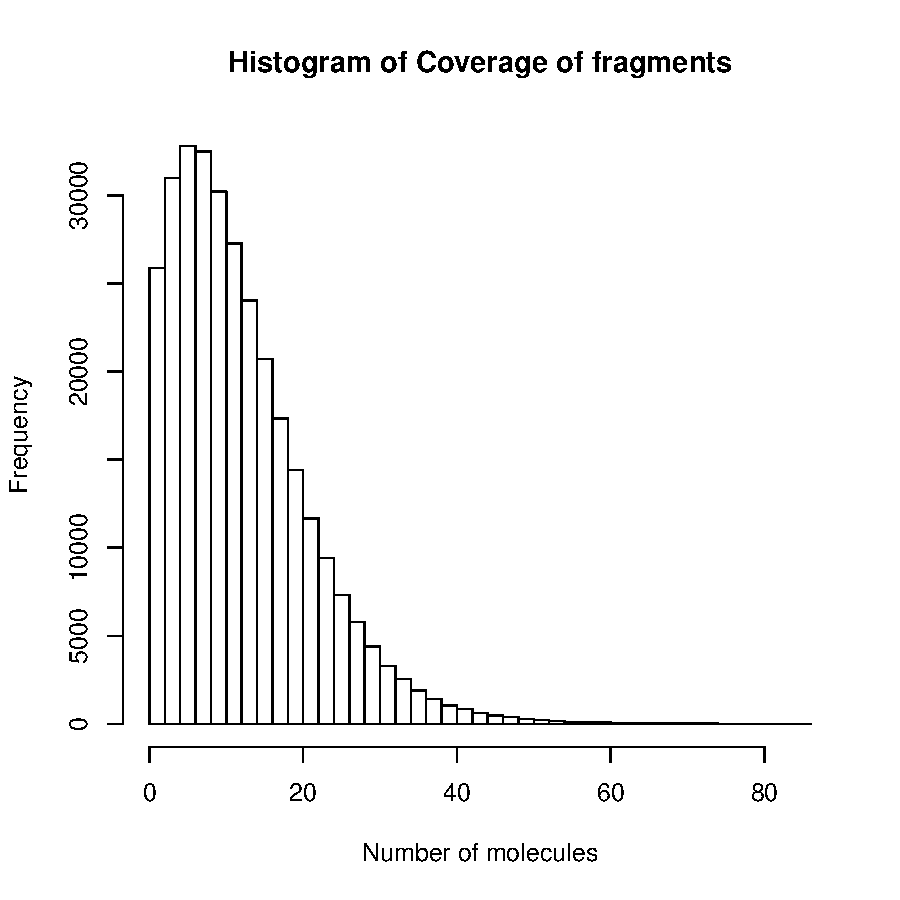
\includegraphics{GCvsIntensity_Report2-003}
% \caption{Some exploratory plots of the Data} % title of Table
\label{fig:Fig1}
\end{figure}

When the variable $intensity\_mean$ is regressed with $fractionGC\_mean$ (or $GC-content$), the coefficient is quite significant (with p-value $<e^{-16}$, but the overall $R^2$ is only $2.5\%$. Similary, $intensity\_sd$ also has a significant relationship with $GC-content$, but the model $R^2$ is quite poor. There is evidence of a positive relationship between fluoroscence intensity and GC-content, however, more in-depth analysis is required. 

\section{Step 2: Modeling intensity and GC-content}
\subsection{With 'GROUP' effect}
As per Prof. Schwartz's suggestion, the following analysis is conducted on the original dataset trimmmed down to only those fragments that have at least 40 molecules aligned to the same genomic location. This trimmed dataset has $35,040$ molecules and $4,513$ groups. The following model includes {\emph{numFrags}}, {\emph{numPixels}} and effect of {\emph{group}} as control variables, when trying to explain the relationship between {\emph{intensity}} and {\emph{gc\_content}}:
$Model4:\\ Y = log(intensity) \\ X = gc\_content + numFrags + as.factor(groupID) + numPixels$ \\
numPixels is a measure of the length (or size) of the molecule. Higher the number of pixels, longer the molecule. 
\\
Below is part of the R-output of the above mentioned model:\\
\noindent
{\bf{\underline{Summary of Model 4}}}
\begin{Schunk}
\begin{Soutput}
                Estimate   Std. Error    t value    Pr(>|t|)
(Intercept) 1.040686e+01 4.844157e-02 214.833244 0.000000000
fractionGC  1.689447e-01 4.097489e-03  41.231277 0.000000000
numFrags    9.119976e-05 4.320786e-05   2.110721 0.034797741
numPixels   2.630645e-06 8.440152e-07   3.116822 0.001828429
\end{Soutput}
\begin{Soutput}
[1] "R-Squared of Model 4:"
\end{Soutput}
\begin{Soutput}
[1] 0.6005516
\end{Soutput}
\end{Schunk}
Introducing the groups as factors seem to explain $60\%$ of the variability. Interestingly, the relationship between fluoroscence intensity and gc\_content remains significant even after introducing the group level effects. The coefficient ($\beta$) of gc\_content is quite stable around $0.17$, both before and after controlling for the other variables. This fact is quite encouraging. The effect of the other variable, like length (or size) of molecule, the number of fragments a molecule is divided into, have small, but statistically significant effect on the explanatory variable. Hence, those variables are not ommitted from the model yet. The relationship, thus far, can be mathematically expressed as (on an average):
\begin{equation}
log(Intensity) = 10.41 + 0.17(GC\_Content) + Other\ Factors
\end{equation}
This relationship is illustrated in the second plot of the other file attached. The red line confirms a positive relationship between intensity and gc-content, after controlling for group effects and other variables.
%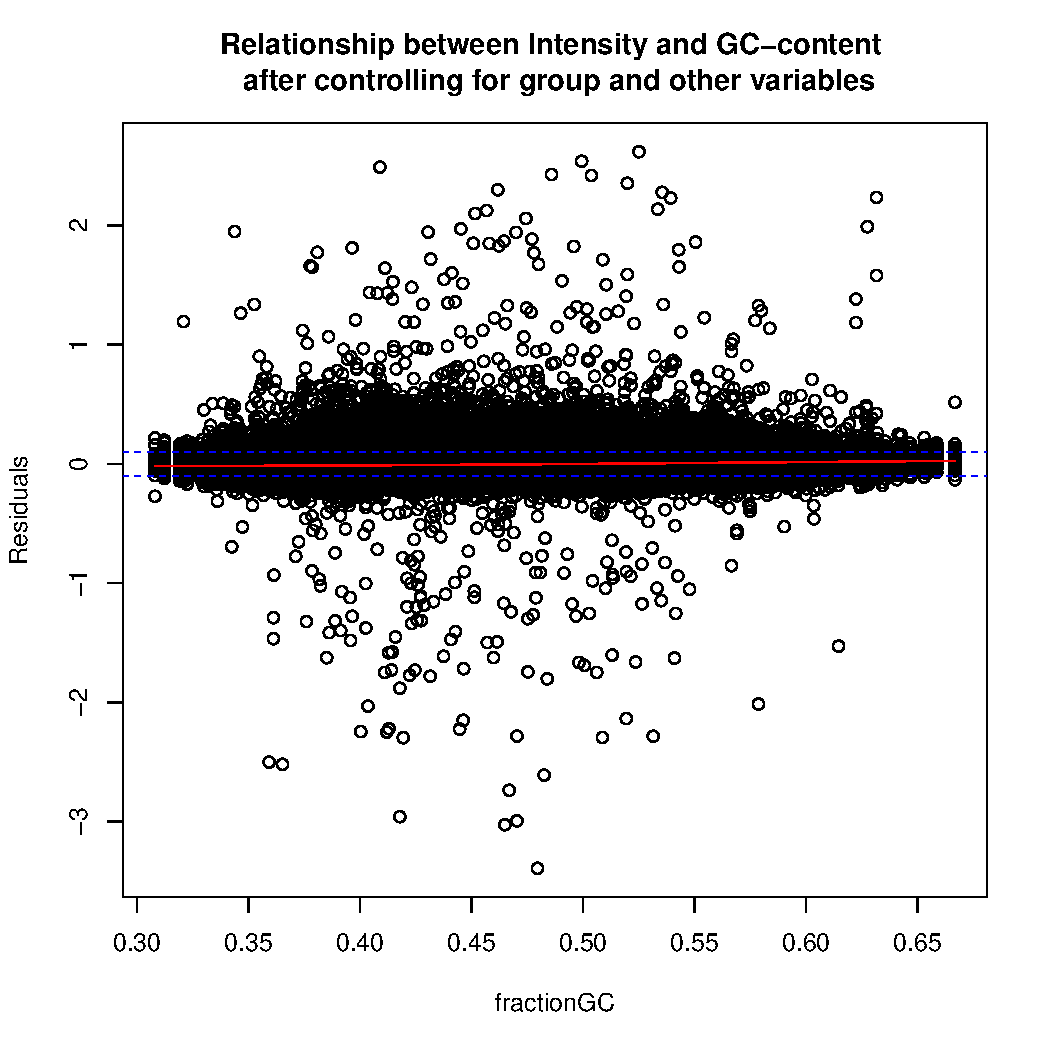
\includepdf[pages={-}]{AVPlot_fractionGC_Model4.pdf}

\subsection{Next Steps}
As per Prof. Newton's suggestions, following are the immediate next steps:
\begin{enumerate}
\item
Fit a weighted least square regression model of the whole dataset; instead of eliminating the fragments with fewer molecules aligned to the same genomic location, this approach would just reduce the weightage. However, this means the design matrix will approximately have 3.8 million rows and around 5,000 columns (based on the number of groups). After trying to run this multiple times, even on a server with 128Gigs RAM, R could not fit the model. Hence, the model estimation has to be broken down by selecting independent subsets of the big dataset. This will be the topic of the next report. This will involve smart parallelly execuble model fitting and subsequent statistical aggregation of the fit between intensity and gc-content.
\item
There could be a contagion effect between fragments next to each other. This effect, if present, should be estimated and subsequently controlled for, before the final model is proposed. This effect could be captured by fitting the model on a molecular level, not on a fragment level. 
\item
Once these effects are controlled for, it would be appropriate to extend the analyses to even shorter fragments (i.e., subdividing the fragments into shorter pieces) and move towards {\emph{intensity signal analysis}}.

\end{enumerate}
The following analysis is conducted on the original dataset, with all the fragments, but higher \end{document}
